\documentclass[11pt]{article}
\usepackage[margin=2.1cm]{geometry}
\usepackage{amsmath,amssymb,booktabs,tikz}
\usepackage{pgfplots}
\pgfplotsset{compat=1.17}
\usepackage[colorlinks=true,linkcolor=blue!55!black]{hyperref}
\usepackage{parskip}
\usetikzlibrary{positioning,arrows.meta,shapes.geometric,shapes.misc,calc,decorations.pathmorphing,fit}

\newcommand{\ve}{v_{\text{ex}}}
\newcommand{\gz}{g_0}
\newcommand{\he}{\ensuremath{{}^3\mathrm{He}}}
\newcommand{\unit}[1]{\,\mathrm{#1}}

\title{\textbf{ORION-Class Torch Ship}\\[3pt]\large Systems, Reactor Physics, and Programme Plan}
\author{}\date{}

% ---------------- symbol library (Apollo-manual conventions) ----------------
\tikzset{
  every picture/.style={line width=0.6pt},
  blk/.style={draw,rectangle,minimum height=7mm,minimum width=15mm,align=center,font=\tiny},
  tank/.style={draw,rounded rectangle,minimum height=9mm,minimum width=17mm,align=center,font=\tiny},
  sph/.style={draw,circle,minimum size=9mm,align=center,font=\tiny},
  pump/.style={draw,circle,minimum size=7mm,inner sep=0,font=\tiny},
  load/.style={draw,rectangle,minimum height=6mm,minimum width=13mm,align=center,font=\tiny,fill=gray!8},
  rad/.style={draw,rectangle,minimum height=8mm,minimum width=26mm,align=center,font=\tiny,fill=blue!4},
  hx/.style={draw,rectangle,minimum height=8mm,minimum width=11mm,align=center,font=\tiny,fill=orange!8},
  thr/.style={draw,isosceles triangle,minimum height=4mm,minimum width=4mm,inner sep=0.5pt},
  lbl/.style={font=\tiny,inner sep=1pt},
  tiny/.style={font=\tiny},
  flow/.style={-{Latex[length=1.6mm]},line width=0.7pt},
  bus/.style={line width=1.6pt},
}
% circuit breaker: a gap with a hinged bar
\newcommand{\cbH}[3]{% x, y, label  (horizontal breaker)
  \draw (#1-0.28,#2) -- (#1-0.12,#2);
  \draw (#1+0.12,#2) -- (#1+0.28,#2);
  \draw (#1-0.12,#2) -- ++(0.20,0.16);
  \fill (#1-0.12,#2) circle (0.5pt); \fill (#1+0.12,#2) circle (0.5pt);
  \node[lbl,above=1.2mm] at (#1,#2) {#3};}
\newcommand{\cbV}[3]{% vertical breaker
  \draw (#1,#2-0.28) -- (#1,#2-0.12);
  \draw (#1,#2+0.12) -- (#1,#2+0.28);
  \draw (#1,#2-0.12) -- ++(0.16,0.20);
  \fill (#1,#2-0.12) circle (0.5pt); \fill (#1,#2+0.12) circle (0.5pt);
  \node[lbl,right=1.0mm] at (#1,#2) {#3};}
% manual valve: bowtie
\newcommand{\valve}[3]{
  \draw[fill=white] (#1-0.13,#2-0.13)--(#1-0.13,#2+0.13)--(#1+0.13,#2-0.13)--(#1+0.13,#2+0.13)--cycle;
  \node[lbl,above=1.0mm] at (#1,#2) {#3};}
% check valve: triangle against a bar
\newcommand{\chk}[3]{
  \draw[fill=white] (#1-0.12,#2-0.12)--(#1-0.12,#2+0.12)--(#1+0.10,#2)--cycle;
  \draw (#1+0.11,#2-0.13)--(#1+0.11,#2+0.13);
  \node[lbl,above=1.2mm] at (#1,#2) {#3};}
% regulator
\newcommand{\reg}[3]{
  \draw[fill=white] (#1-0.16,#2-0.14) rectangle (#1+0.16,#2+0.14);
  \draw (#1-0.16,#2-0.14)--(#1+0.16,#2+0.14);
  \node[lbl,above=1.6mm] at (#1,#2) {#3};}


\begin{document}
\maketitle
\vspace{-2.4em}
\begin{center}\small Technical reference, revision 2 --- with the fusion plant worked from first principles.\end{center}
\hrule
\tableofcontents
\hrule
\vspace{0.8em}

\section{The ship at a glance}
ORION is a $\sim$650\,t fusion-torch vessel that crosses to Mars in about six days at $0.30\,\gz$ sustained acceleration. The design is driven by three hard constraints, discovered in that order:
\begin{enumerate}\itemsep1pt
\item \textbf{Drive specific power} sets the top speed. Before heat or radiation bind, the \emph{mass closure loop} diverges: too much acceleration and no finite ship exists.
\item \textbf{The radiator sets the cruise, not the engine.} Rejecting waste heat by $T^4$ radiation alone demands enormous area.
\item \textbf{Fast transit is itself radiation shielding.} A six-day crossing cuts galactic-cosmic-ray dose $\sim$40$\times$ versus a Hohmann transfer.
\end{enumerate}

\begin{center}
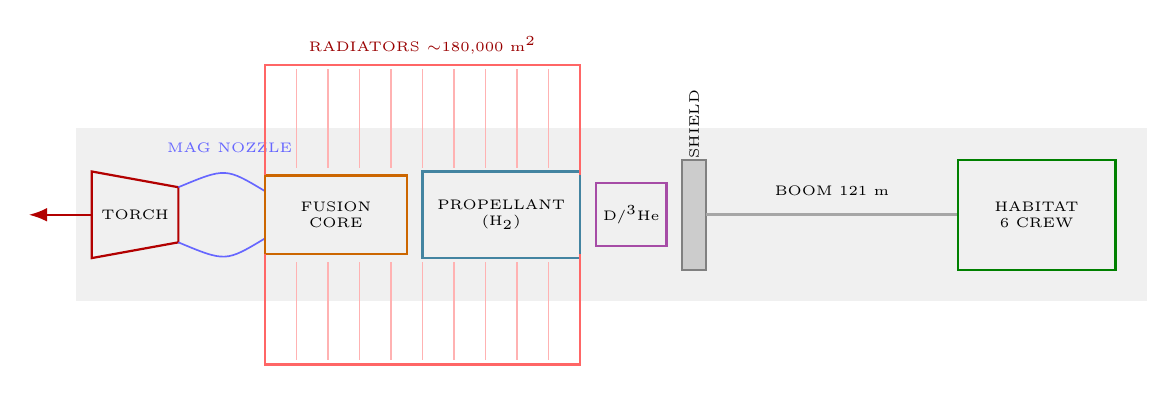
\begin{tikzpicture}[font=\scriptsize,>=Latex]
\fill[gray!12] (0,-1.1) rectangle (13.6,1.1);
% torch
\draw[thick,red!70!black] (0.2,-0.55) -- (1.3,-0.35) -- (1.3,0.35) -- (0.2,0.55) -- cycle;
\node at (0.75,0) {\tiny TORCH};
\draw[->,red!70!black,thick] (0.2,0) -- (-0.6,0);
% magnetic nozzle
\draw[blue!60] (1.3,0.35) .. controls (1.9,0.6) .. (2.4,0.3);
\draw[blue!60] (1.3,-0.35) .. controls (1.9,-0.6) .. (2.4,-0.3);
\node[blue!60] at (1.95,0.85) {\tiny MAG NOZZLE};
% reactor
\draw[thick,orange!80!black] (2.4,-0.5) rectangle (4.2,0.5);
\node[align=center] at (3.3,0) {\tiny FUSION\\[-2pt]\tiny CORE};
% propellant + fuel tanks
\draw[thick,cyan!60!black] (4.4,-0.55) rectangle (6.4,0.55);
\node[align=center] at (5.4,0) {\tiny PROPELLANT\\[-2pt]\tiny (H$_2$)};
\draw[thick,violet!70] (6.6,-0.4) rectangle (7.5,0.4);
\node[align=center] at (7.05,0) {\tiny D/$^3$He};
% radiators
\draw[thick,red!60] (2.4,0.5) -- (2.4,1.9) -- (6.4,1.9) -- (6.4,0.5);
\draw[thick,red!60] (2.4,-0.5) -- (2.4,-1.9) -- (6.4,-1.9) -- (6.4,-0.5);
\foreach \x in {2.8,3.2,...,6.2} {\draw[red!30] (\x,0.6)--(\x,1.85); \draw[red!30] (\x,-0.6)--(\x,-1.85);}
\node[red!60!black] at (4.4,2.15) {\tiny RADIATORS $\sim$180{,}000 m$^2$};
% shadow shield
\draw[thick,gray,fill=gray!40] (7.7,-0.7) rectangle (8.0,0.7);
\node[rotate=90] at (7.85,1.15) {\tiny SHIELD};
% boom
\draw[very thick,gray!70] (8.0,0) -- (11.2,0);
\node at (9.6,0.3) {\tiny BOOM 121 m};
% hab
\draw[thick,green!50!black] (11.2,-0.7) rectangle (13.2,0.7);
\node[align=center] at (12.2,0) {\tiny HABITAT\\[-2pt]\tiny 6 CREW};
\end{tikzpicture}
\end{center}

\section{The reactor: what it burns and how it works}

\subsection{Why fusion, and which reaction}
Four candidate reactions matter. The choice is a three-way fight between \emph{how hard it is to ignite}, \emph{how many neutrons it throws}, and \emph{whether the energy comes out as charged particles you can use directly}.

\begin{center}\small
\begin{tabular}{@{}llrrl@{}}
\toprule
Reaction & Products & Energy & Neutron share & Ignition $T$\\
\midrule
D + T $\to$ $^4$He + n & 3.5 + 14.1 MeV & 17.6 MeV & \textbf{80\%} & $\sim$15 keV\\
D + D $\to$ (two branches) & p+T / n+$^3$He & 3.7 / 3.3 MeV & $\sim$50\% & $\sim$50 keV\\
\textbf{D + \he\ $\to$ $^4$He + p} & \textbf{3.6 + 14.7 MeV} & \textbf{18.3 MeV} & \textbf{$\sim$0\%*} & $\sim$60 keV\\
p + $^{11}$B $\to$ 3\,$^4$He & 8.7 MeV & 8.7 MeV & 0\% & $\sim$150 keV\\
\bottomrule
\end{tabular}
\end{center}
\noindent{\footnotesize *nominally --- see \S2.5, the neutron caveat.}

\textbf{ORION burns deuterium and helium-3.}
\begin{equation}
\mathrm{D} + \he \;\longrightarrow\; {}^4\mathrm{He}\,(3.6\unit{MeV}) \;+\; \mathrm{p}\,(14.7\unit{MeV}),
\qquad Q = 18.3\unit{MeV}.
\end{equation}
The decisive property is that \textbf{both products are electrically charged}. A charged exhaust can be steered by a magnetic nozzle (so it becomes \emph{thrust} directly), and charged particles can be decelerated against an electric field to recover power \emph{without a heat engine}. Neither is possible with D--T, whose energy leaves as 14.1 MeV neutrons: neutrons cannot be magnetically steered, cannot be directly converted, and activate the structure. A D--T torch would be a neutron lamp bolted to a heat exchanger.

The price is difficulty. Specific energy is
\begin{equation}
\frac{Q}{m_{\mathrm{D}}+m_{\he}}=\frac{2.932\times10^{-12}\unit{J}}{8.353\times10^{-27}\unit{kg}}
= 3.51\times10^{14}\unit{J/kg},
\end{equation}
about ten million times chemical fuel --- but it must be lit at hundreds of millions of kelvin.

\subsection{Reactivity: the price of going aneutronic}
The fusion power density depends on the \emph{reactivity} $\langle\sigma v\rangle$, the velocity-averaged cross-section:
\begin{equation}
P_{\text{fus}} = n_1 n_2 \,\langle\sigma v\rangle\, Q \qquad [\mathrm{W/m^3}].
\end{equation}
The curves below are computed from the Bosch--Hale parametrization (not sketched):

\begin{center}
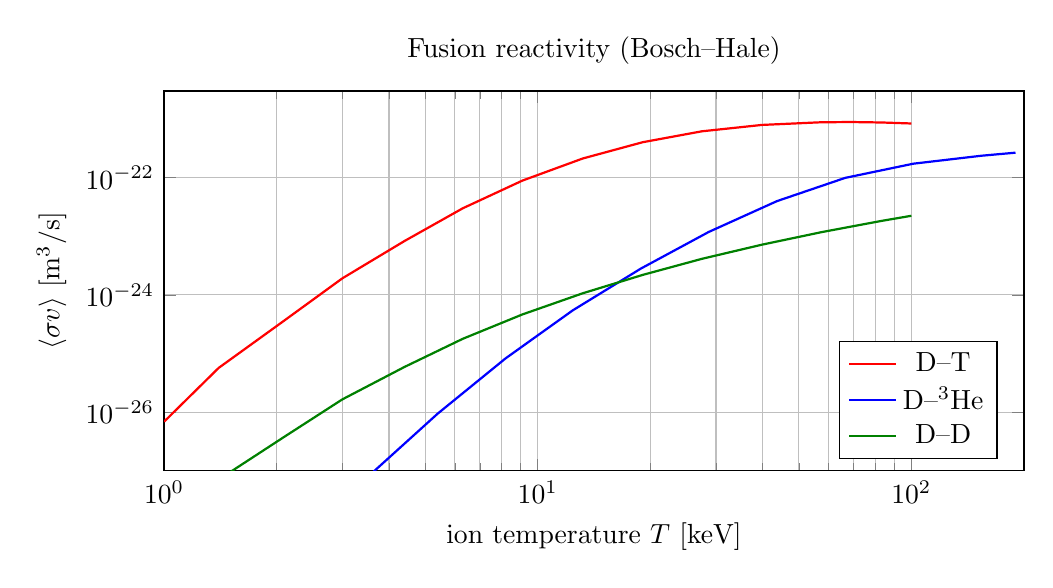
\begin{tikzpicture}
\begin{axis}[width=12.5cm,height=6.4cm,xmode=log,ymode=log,
  xlabel={ion temperature $T$ [keV]}, ylabel={$\langle\sigma v\rangle$ [m$^3$/s]},
  xmin=1,xmax=200,ymin=1e-27,ymax=3e-21,grid=both,legend pos=south east,
  title={Fusion reactivity (Bosch--Hale)}]
\addplot[thick,red] coordinates {(1.0,6.857e-27)(1.4,5.678e-26)(2.1,3.672e-25)(3.0,1.920e-24)(4.4,8.323e-24)(6.3,3.011e-23)(9.1,8.949e-23)(13.2,2.134e-22)(19.1,4.046e-22)(27.5,6.212e-22)(39.8,7.980e-22)(57.5,8.870e-22)(69.2,8.942e-22)(83.2,8.788e-22)(100.0,8.448e-22)};
\addlegendentry{D--T}
\addplot[thick,blue] coordinates {(1.0,3.057e-32)(1.5,1.490e-30)(2.3,4.263e-29)(3.5,7.714e-28)(5.4,9.422e-27)(8.2,8.239e-26)(12.4,5.434e-25)(18.9,2.826e-24)(28.7,1.190e-23)(43.7,3.998e-23)(66.5,9.951e-23)(101.2,1.739e-22)(154.0,2.378e-22)(190.0,2.682e-22)};
\addlegendentry{D--$^3$He}
\addplot[thick,green!50!black] coordinates {(1.0,1.017e-28)(1.4,7.040e-28)(2.1,3.801e-27)(3.0,1.648e-26)(4.4,5.894e-26)(6.3,1.781e-25)(9.1,4.644e-25)(13.2,1.067e-24)(19.1,2.197e-24)(27.5,4.131e-24)(39.8,7.201e-24)(57.5,1.180e-23)(83.2,1.835e-23)(100.0,2.244e-23)};
\addlegendentry{D--D}
\end{axis}
\end{tikzpicture}
\end{center}

At its peak D--T reaches $8.9\times10^{-22}\unit{m^3/s}$ near 67 keV; D--\he\ manages only $2.7\times10^{-22}$ and needs $\sim$190 keV to get there. \textbf{D--\he\ is roughly $3\times$ less reactive and needs $3\times$ the temperature.} That is exactly what we pay for a charged-particle exhaust, and it is why the plant runs at $T_{\text{ion}}\approx10$--15 keV during ramp-up but must be driven far hotter to reach full gain.

\subsection{Ignition: the Lawson criterion}
Fusion self-sustains when the power deposited by charged products exceeds losses. In the standard form, the \emph{triple product} must exceed a threshold:
\begin{equation}
\boxed{\;n\,T\,\tau_E \;\gtrsim\; \text{const.}\;}
\end{equation}
where $n$ is density, $T$ temperature, $\tau_E$ the energy confinement time. Approximate requirements:
\begin{center}\small
\begin{tabular}{@{}lrr@{}}
\toprule
Fuel & $nT\tau_E$ [keV$\cdot$s/m$^3$] & optimum $T$\\
\midrule
D--T   & $\sim3\times10^{21}$ & 15 keV\\
D--\he & $\sim1\times10^{23}$ & 60 keV\\
p--$^{11}$B & $\sim3\times10^{24}$ & 150 keV\\
\bottomrule
\end{tabular}
\end{center}
D--\he\ is $\sim$30$\times$ harder to ignite than D--T. This is the single fictional concession the setting makes: ORION's plant achieves a D--\he\ triple product that real machines have not.

The \textbf{gain} $Q$ tracked on the reactor panel is
\begin{equation}
Q = \frac{P_{\text{fusion}}}{P_{\text{external heating}}},
\end{equation}
so $Q=1$ is breakeven and $Q\to\infty$ is full ignition. The simulator treats $Q>5$ as \emph{self-sustaining}: at that point the RF heaters back off and the burn carries itself. That threshold is why the ignition sequence has a distinct \textsc{ignite}$\to$\textsc{ascent} transition.

\subsection{Confinement and the magnets}
The plasma is held off the walls by a toroidal magnetic field. Two numbers matter.

\textbf{Plasma beta} --- the ratio of plasma pressure to magnetic pressure:
\begin{equation}
\beta=\frac{2\mu_0 nkT}{B^2}.
\end{equation}
Confinement fails above a critical $\beta$, so higher $B$ permits higher density and thus more power. This is why the machine wants 8 T.

\textbf{Stored magnetic energy} --- the reason a quench is catastrophic:
\begin{equation}
u=\frac{B^2}{2\mu_0}, \qquad E_{\text{coil}}=\frac{B^2}{2\mu_0}V .
\end{equation}
At $B=8\unit{T}$, $u=25.5\unit{MJ/m^3}$. With a field volume of $\sim$12\,m$^3$ the coils store
\begin{equation}
E_{\text{coil}} \approx 306\unit{MJ},
\end{equation}
consistent with the simulator's 4 MW charging over a 75-second ramp ($4\times10^6 \times 75 = 300$ MJ). \textbf{That is the energy of $\sim$70 kg of TNT stored in the magnets.}

\subsection{The neutron caveat --- why we still carry a shield}
D--\he\ is called ``aneutronic,'' but a deuterium plasma inevitably burns \emph{itself}:
\begin{equation}
\mathrm{D}+\mathrm{D}\to\mathrm{n}\,(2.45\unit{MeV})+\he \qquad(\sim50\%\text{ of D--D events}).
\end{equation}
These side reactions typically put a few percent of total power into neutrons. Small compared to D--T's 80\%, but not zero --- which is precisely why ORION still needs the 121\,m boom and the 16\,cm shadow shield derived in the shielding analysis. \textbf{The fuel choice shrinks the shield; it does not delete it.}

\subsection{Fuel supply --- a plot hook that is also physics}
Deuterium is trivial: 1 atom in 6400 of hydrogen, so seawater is an inexhaustible source. \textbf{Helium-3 is the problem.} It is essentially absent on Earth (the geomagnetic field deflects the solar wind that makes it). The two real reservoirs are:
\begin{itemize}\itemsep0pt
\item \textbf{Lunar regolith} --- implanted by 4 billion years of solar wind, at $\sim$10--20 parts per \emph{billion}. Extracting one tonne means processing $\sim$10$^8$ tonnes of soil.
\item \textbf{Gas giant atmospheres} --- Jupiter and Saturn are rich in it, but require aerocapture mining.
\end{itemize}
ORION burns $\sim$27 grams of fuel per second (\S3.2). That sounds trivial --- but the \he\ half of it is the most expensive substance in the solar system, and this alone explains why a civilisation with torch drives would care intensely about the Moon and the outer planets.

\subsection{Startup sequence --- the physics behind each stage}
\begin{center}\small
\begin{tabular}{@{}llll@{}}
\toprule
Stage & Physics & Gate to advance & Failure mode\\
\midrule
\textsc{pumpdown} & evacuate chamber, $p\propto e^{-t/\tau}$ & $p<10^{-3}$ Pa & impurities quench burn\\
\textsc{field} & charge coils, $E=\tfrac{B^2}{2\mu_0}V$ & $I=50$ kA, $B=8$ T & \textbf{coil quench}\\
\textsc{heat} & gas puff + RF heating & $T_i\ge10$ keV, $n\ge1.0$ & density disruption\\
\textsc{ignite} & gain climbs, $Q=P_{\text{fus}}/P_{\text{ext}}$ & $Q\ge5$ & vacuum/field loss\\
\textsc{ascent} & thermal power ramps to 50 MW & $P_{\text{th}}=50$ MW & coolant overtemp\\
\textsc{online} & 20 MW$_e$ steady & --- & scram on overtemp\\
\bottomrule
\end{tabular}
\end{center}

\textbf{Quench} deserves its own paragraph, because it is the reason cooling must precede ignition. A superconductor carries current with zero resistance only below a critical surface in ($T$, $B$, $J$). If any part of the winding warms past $T_c$, that spot goes \emph{normal} --- it acquires resistance, ohmic heating $I^2R$ dumps energy locally, the normal zone propagates, and the coil tries to dissipate its \emph{entire} 306 MJ into a small volume of metal. The magnet destroys itself. Hence the simulator's rule: no coolant flow during \textsc{field} $\Rightarrow$ coil temperature climbs $\Rightarrow$ quench abort at 40 K.

\subsection{Power conversion}
Because the products are charged, two paths exist:
\begin{align}
\text{Thermal cycle:}\quad & \eta \approx 0.35\text{--}0.45 \quad(\text{blanket}\to\text{turbine}) \\
\text{Direct conversion:}\quad & \eta \approx 0.6\text{--}0.8 \quad(\text{decelerate ions against a field})
\end{align}
ORION's \emph{housekeeping} reactors use a thermal cycle at $\eta=0.40$ (50 MW$_{\text{th}}\to$ 20 MW$_e$, 30 MW waste heat --- which is exactly the heat load the coolant loop must reject). The \emph{main torch} needs no conversion at all: the plasma is simply exhausted through a magnetic nozzle. This is why the two loops are modelled separately.

\section{The torch: mass augmentation (a system we have not yet modelled)}

\subsection{From fusion products to thrust}
If the plasma were exhausted directly, its velocity would follow from the reaction energy:
\begin{equation}
v_{\text{prod}}=\sqrt{\frac{2Q}{m_{\mathrm{D}}+m_{\he}}}
=\sqrt{\frac{2(2.932\times10^{-12})}{8.353\times10^{-27}}}
=2.65\times10^{7}\unit{m/s},
\end{equation}
which is $8.8\%$ of light speed --- an $I_{sp}$ of $2.7\times10^{6}$ s.

\textbf{But ORION's design $\ve$ is $9.81\times10^{6}$ m/s ($I_{sp}=10^{6}$ s) --- deliberately \emph{lower}.} Why throw away performance?

\subsection{The reason: thrust is bought by diluting the exhaust}
For a \emph{fixed} jet power $P$,
\begin{equation}
P=\tfrac12\dot m\,\ve^{2}=\tfrac12 F\,\ve
\qquad\Longrightarrow\qquad
\boxed{\;F=\frac{2P}{\ve}\;}
\end{equation}
Thrust is \emph{inversely} proportional to exhaust velocity. A pure-fusion-product exhaust is magnificently efficient and nearly useless for pushing a 650-tonne ship: you would get a third of the thrust. So the drive \textbf{injects inert propellant (hydrogen) into the plasma stream}, which shares the energy, slows the exhaust, and multiplies the thrust. Energy conservation fixes the mixing ratio exactly:
\begin{equation}
\tfrac12\dot m_{\text{tot}}\ve^{2}=\tfrac12\dot m_{\text{fuel}}v_{\text{prod}}^{2}
\qquad\Longrightarrow\qquad
\boxed{\;\frac{\dot m_{\text{tot}}}{\dot m_{\text{fuel}}}=\left(\frac{v_{\text{prod}}}{\ve}\right)^{2}\;}
\end{equation}

\textit{At the design point:} $(2.65\times10^{7}/9.81\times10^{6})^{2}=\mathbf{7.30}$. And independently, from the mass flows: $\dot m_{\text{tot}}=F/\ve=0.195\unit{kg/s}$, while the fuel burn needed to make 9.37 TW is $\dot m_{\text{fuel}}=P/(Q/m)=9.37\times10^{12}/3.51\times10^{14}=0.0267\unit{kg/s}$. Ratio: $0.195/0.0267=\mathbf{7.30}$. \emph{The two derivations agree exactly} --- the model is self-consistent.

\begin{center}
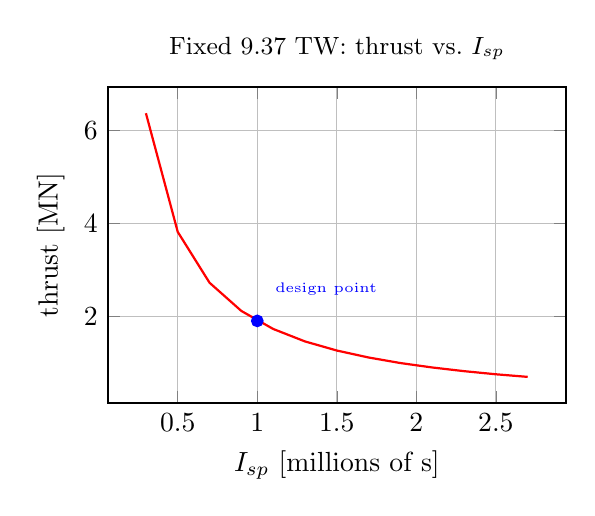
\begin{tikzpicture}
\begin{axis}[width=7.4cm,height=5.6cm,xlabel={$I_{sp}$ [millions of s]},ylabel={thrust [MN]},
  grid=both,title={\small Fixed 9.37 TW: thrust vs.\ $I_{sp}$}]
\addplot[thick,red] coordinates {(0.30,6.368)(0.50,3.821)(0.70,2.729)(0.90,2.123)(1.10,1.737)(1.30,1.469)(1.50,1.274)(1.70,1.124)(1.90,1.005)(2.10,0.910)(2.30,0.831)(2.50,0.764)(2.70,0.708)};
\addplot[only marks,mark=*,blue] coordinates {(1.0,1.91)};
\node[blue,anchor=west,font=\tiny] at (axis cs:1.05,2.6) {design point};
\end{axis}
\end{tikzpicture}
\hfill
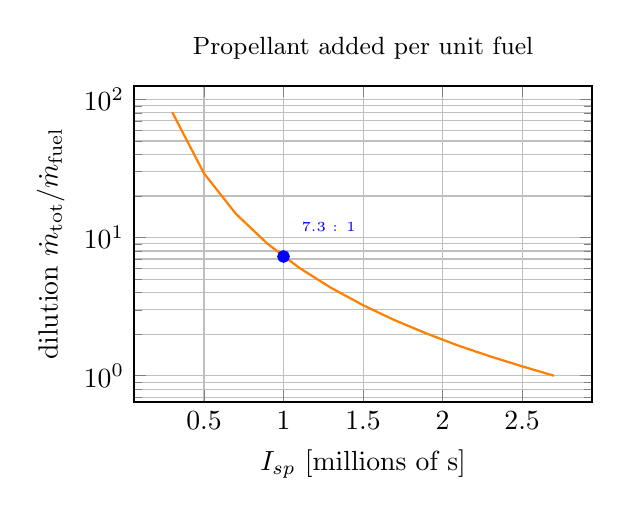
\begin{tikzpicture}
\begin{axis}[width=7.4cm,height=5.6cm,xlabel={$I_{sp}$ [millions of s]},ylabel={dilution $\dot m_{\text{tot}}/\dot m_{\text{fuel}}$},
  ymode=log,grid=both,title={\small Propellant added per unit fuel}]
\addplot[thick,orange] coordinates {(0.30,81.06)(0.50,29.18)(0.70,14.89)(0.90,9.01)(1.10,6.03)(1.30,4.32)(1.50,3.24)(1.70,2.52)(1.90,2.02)(2.10,1.65)(2.30,1.38)(2.50,1.17)(2.70,1.00)};
\addplot[only marks,mark=*,blue] coordinates {(1.0,7.30)};
\node[blue,anchor=west,font=\tiny] at (axis cs:1.05,12) {7.3 : 1};
\end{axis}
\end{tikzpicture}
\end{center}

\begin{center}
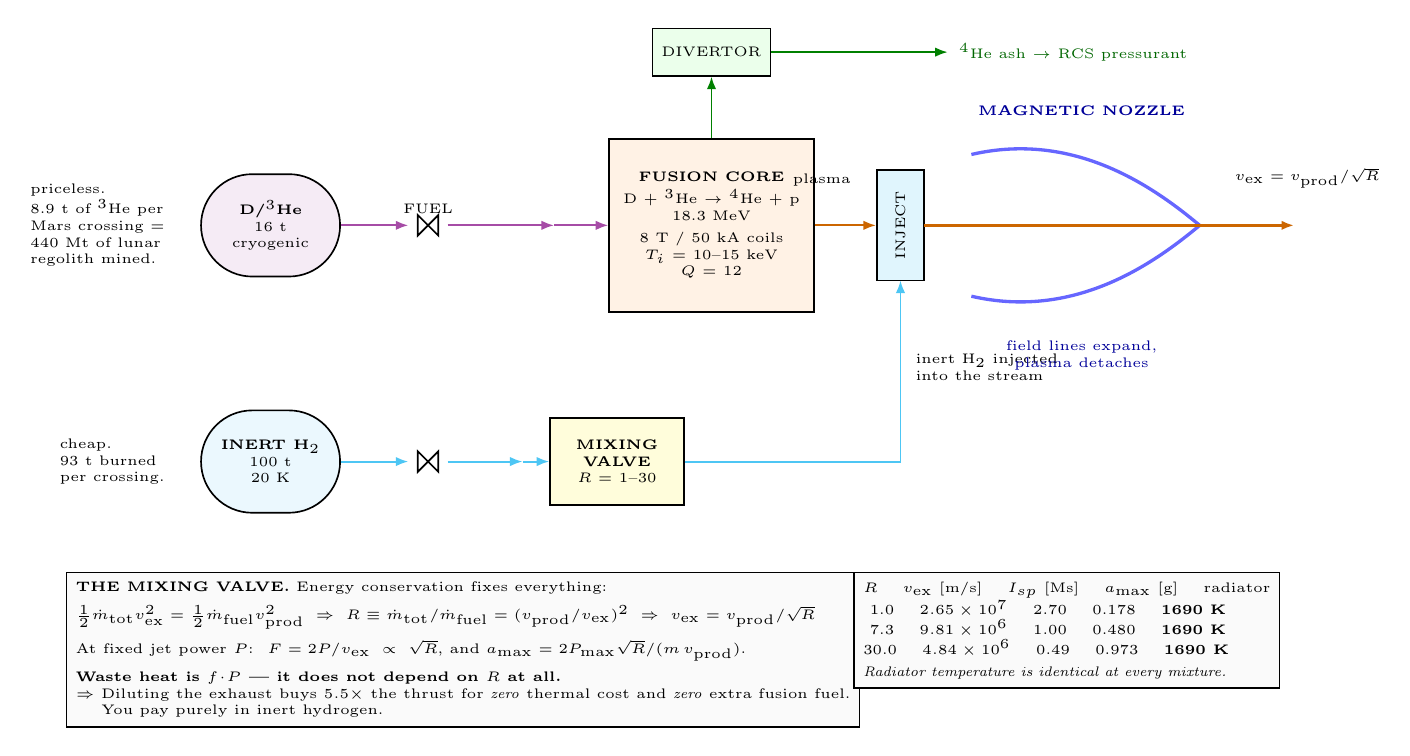
\begin{tikzpicture}[x=1cm,y=1cm]
% fuel flask
\node[tank,minimum width=20mm,minimum height=13mm,fill=violet!8] (FL) at (0,3.4)
  {\textbf{D/$^3$He}\\16 t\\cryogenic};
\node[lbl,align=left,anchor=east] at (-1.3,3.4) {priceless.\\8.9 t of $^3$He per\\Mars crossing =\\440 Mt of lunar\\regolith mined.};
% inert tank
\node[tank,minimum width=20mm,minimum height=13mm,fill=cyan!8] (H2) at (0,0.4)
  {\textbf{INERT H$_2$}\\100 t\\20 K};
\node[lbl,align=left,anchor=east] at (-1.3,0.4) {cheap.\\93 t burned\\per crossing.};
% fuel feed
\valve{2.0}{3.4}{FUEL}
\draw[flow,violet!70] (FL.east) -- (1.75,3.4);
\draw[flow,violet!70] (2.25,3.4) -- (3.6,3.4);
% inert feed + MIXING VALVE
\valve{2.0}{0.4}{}
\draw[flow,cyan!70] (H2.east) -- (1.75,0.4);
\draw[flow,cyan!70] (2.25,0.4) -- (3.2,0.4);
\node[blk,minimum width=17mm,minimum height=11mm,fill=yellow!14] (MIX) at (4.4,0.4)
  {\textbf{MIXING}\\\textbf{VALVE}\\$R$ = 1--30};
\draw[flow,cyan!70] (3.2,0.4) -- (MIX.west);
% reactor core
\node[blk,minimum width=26mm,minimum height=22mm,fill=orange!10] (CORE) at (5.6,3.4)
  {\textbf{FUSION CORE}\\[2pt] D + $^3$He $\to$ $^4$He + p\\ 18.3 MeV\\[2pt] 8 T / 50 kA coils\\ $T_i$ = 10--15 keV\\ $Q$ = 12};
\draw[flow,violet!70] (3.6,3.4) -- (CORE.west);
% injection ring
\node[blk,minimum width=6mm,minimum height=14mm,fill=cyan!12] (INJ) at (8.0,3.4) {\rotatebox{90}{INJECT}};
\draw[flow,orange!80!black] (CORE.east) -- (INJ.west);
\node[lbl,above] at (7.0,3.85) {plasma};
\draw[flow,cyan!70] (MIX.east) -- (8.0,0.4) -- (8.0,2.7);
\node[lbl,right,align=left] at (8.15,1.6) {inert H$_2$ injected\\into the stream};
% magnetic nozzle
\draw[line width=1.2pt,blue!60] (8.9,4.3) .. controls (10.2,4.6) and (11.2,3.9) .. (11.8,3.4);
\draw[line width=1.2pt,blue!60] (8.9,2.5) .. controls (10.2,2.2) and (11.2,2.9) .. (11.8,3.4);
\node[lbl,blue!60!black] at (10.3,4.85) {\textbf{MAGNETIC NOZZLE}};
\node[lbl,blue!60!black,align=center] at (10.3,1.75) {field lines expand,\\plasma detaches};
\draw[flow,orange!80!black,line width=1.3pt] (8.3,3.4) -- (13.0,3.4);
\node[lbl,align=left,anchor=west] at (12.2,4.0) {$v_{\text{ex}} = v_{\text{prod}}/\sqrt{R}$};
% divertor -> he scavenge
\node[blk,minimum width=13mm,minimum height=6mm,fill=green!8] (DIV) at (5.6,5.6) {DIVERTOR};
\draw[flow,green!50!black] (CORE.north) -- (DIV.south);
\draw[flow,green!50!black] (DIV.east) -- (8.6,5.6);
\node[lbl,green!40!black,right] at (8.7,5.6) {$^4$He ash $\to$ RCS pressurant};
% equations box
\node[draw,align=left,font=\tiny,anchor=north west,fill=gray!4] at (-2.6,-1.0)
 {\textbf{THE MIXING VALVE.} Energy conservation fixes everything:\\[3pt]
  $\tfrac12 \dot m_{\text{tot}} v_{\text{ex}}^2 = \tfrac12 \dot m_{\text{fuel}} v_{\text{prod}}^2
   \;\Rightarrow\; R \equiv \dot m_{\text{tot}}/\dot m_{\text{fuel}} = (v_{\text{prod}}/v_{\text{ex}})^2
   \;\Rightarrow\; v_{\text{ex}} = v_{\text{prod}}/\sqrt{R}$\\[3pt]
  At fixed jet power $P$: $\;F = 2P/v_{\text{ex}} \;\propto\; \sqrt{R}$, and $a_{\max} = 2P_{\max}\sqrt{R}/(m\,v_{\text{prod}})$.\\[3pt]
  \textbf{Waste heat is $f\!\cdot\!P$ --- it does not depend on $R$ at all.}\\
  $\Rightarrow$ Diluting the exhaust buys $5.5\times$ the thrust for \emph{zero} thermal cost and \emph{zero} extra fusion fuel.\\
  \phantom{$\Rightarrow$} You pay purely in inert hydrogen.};
\node[draw,align=left,font=\tiny,anchor=north west,fill=gray!4] at (7.4,-1.0)
 {\textbf{$R$} \quad $v_{\text{ex}}$ [m/s] \quad $I_{sp}$ [Ms] \quad $a_{\max}$ [g] \quad radiator\\
  \ 1.0 \quad $2.65\times10^7$ \quad 2.70 \quad 0.178 \quad \textbf{1690 K}\\
  \ 7.3 \quad $9.81\times10^6$ \quad 1.00 \quad 0.480 \quad \textbf{1690 K}\\
  30.0 \quad $4.84\times10^6$ \quad 0.49 \quad 0.973 \quad \textbf{1690 K}\\[2pt]
  \emph{Radiator temperature is identical at every mixture.}};
\end{tikzpicture}
\end{center}

\subsection{The mixing valve is the most important control in the ship}
$R$ is a \textbf{real-time pilot control} that trades $I_{sp}$ against thrust at constant reactor power. Since $\ve=v_{\text{prod}}/\sqrt{R}$ and $F=2P/\ve$, the \emph{maximum attainable acceleration} scales as
\begin{equation}
a_{\max}=\frac{2P_{\max}\sqrt{R}}{m\,v_{\text{prod}}}\;\propto\;\sqrt{R}.
\end{equation}
The simulator's own output, at $P_{\max}=15\unit{TW}$ on a 650\,t ship:

\begin{center}\small
\begin{tabular}{@{}rrrrrr@{}}
\toprule
$R$ & $\ve$ [m/s] & $I_{sp}$ [Ms] & $a_{\max}$ [g] & $\dot m_{\text{fuel}}$ & \textbf{radiator} \\
\midrule
1.0  & $2.650\times10^{7}$ & 2.702 & 0.178 & 0.0427 & \textbf{1690 K}\\
2.0  & $1.874\times10^{7}$ & 1.911 & 0.251 & 0.0427 & \textbf{1690 K}\\
4.0  & $1.325\times10^{7}$ & 1.351 & 0.355 & 0.0427 & \textbf{1690 K}\\
\textbf{7.3} & $9.808\times10^{6}$ & \textbf{1.000} & \textbf{0.480} & 0.0427 & \textbf{1690 K}\\
15.0 & $6.842\times10^{6}$ & 0.698 & 0.688 & 0.0427 & \textbf{1690 K}\\
30.0 & $4.838\times10^{6}$ & 0.493 & 0.973 & 0.0427 & \textbf{1690 K}\\
\bottomrule
\end{tabular}
\end{center}

\textbf{Read the last two columns.} Across a $30\times$ change in mixture, the fusion fuel burn is \emph{identical} and the radiator temperature is \emph{identical}. Waste heat is $f\!\cdot\!P$ --- it depends on the \emph{power}, and the mixing valve does not change the power. So:

\begin{center}\fbox{\parbox{0.9\textwidth}{\centering
\textbf{Diluting the exhaust buys $5.5\times$ the thrust for zero thermal cost and zero extra fusion fuel.\\
You pay for it purely in inert hydrogen.}}}
\end{center}

This is the cleanest trade in the vehicle:
\begin{itemize}\itemsep1pt
\item \textbf{Rich} ($R\to30$): nearly 1 g available. Hard manoeuvring, emergency burns. Drinks the H$_2$ tank.
\item \textbf{Lean} ($R\to1$): $I_{sp}$ of 2.7 million seconds, but only $0.18\,\gz$. Economical cruise; enormous $\Delta v$ reserve.
\item If the commanded acceleration exceeds what the plant can supply, \textbf{the pilot's remedy is to richen the mixture} --- not to demand more power.
\end{itemize}
Two tanks, depleting at different rates: \textbf{100 t of cheap inert hydrogen} and \textbf{16 t of priceless D/\he}. A Mars crossing at the design point burns 93.0 t of the former and 14.8 t of the latter.

\textit{Fuel for a Mars run:} $0.0267\unit{kg/s}\times 5.53\times10^{5}\unit{s}=\mathbf{14.8\,t}$ of D/\he, of which $3/5$ by mass --- $\mathbf{8.9\,t}$ --- is \he. At a lunar regolith concentration of 20 parts per billion, that single crossing represents \textbf{$\sim$440 million tonnes of regolith processed.} The propellant is cheap; the fuel is an industrial programme.

\section{Guidance avionics (after Apollo)}
The Apollo CSM solved these problems, and its failure modes are the interesting ones. ORION copies the architecture.

\subsection{The stable platform, and gimbal lock}
The IMU is a gyro-stabilised platform on three gimbals, holding an inertial reference (the \textsc{refsmmat}) that all guidance is measured against. Gimbals have a fatal geometry: when the \textbf{middle gimbal} rotates far enough, the outer and inner axes become nearly parallel, the platform loses a degree of freedom, and it \textbf{tumbles}. The reference is destroyed.

Apollo lit its \textsc{gimbal lock} warning at $\pm70^\circ$ of middle gimbal. ORION uses the same numbers:
\begin{center}\small
\begin{tabular}{@{}lll@{}}
\toprule
Middle gimbal & State & Consequence\\
\midrule
$<70^\circ$ & normal & ---\\
$70^\circ$--$85^\circ$ & \textsc{gimbal lock} warning & manoeuvre away \emph{now}\\
$>85^\circ$ & \textbf{locked} & platform tumbles; reference \textbf{lost}\\
\bottomrule
\end{tabular}
\end{center}

\subsection{Why there is a second, worse attitude reference}
The \textbf{GDC} integrates the rate gyros instead of holding a platform. It drifts $20\times$ faster (18 vs.\ 0.9 arcmin/hour) --- but \textbf{it has no gimbals, so it cannot lock}. The manoeuvre that destroys the IMU leaves the GDC intact. One button (\textsc{gdc align}) copies the IMU's reference across while you still have it. This is redundancy through \emph{dissimilarity}: not two of the same box, but two boxes that fail differently.

\subsection{Platform alignment (P52)}
Gyros drift, so the platform must be re-aligned against stars. The sequence, and its gates:
\begin{center}\small
\begin{tabular}{@{}lll@{}}
\toprule
Phase & Action & Gate\\
\midrule
\textsc{coarse align} & torque platform roughly into place & rates $<0.05^\circ$/s\\
\textsc{mark 1} & sight first catalogue star & rates $<0.05^\circ$/s\\
\textsc{mark 2} & sight second star & rates $<0.05^\circ$/s\\
\textsc{star angle diff} & compare measured vs.\ catalogued separation & within limits, else \textbf{reject}\\
\textsc{torquing} & apply computed torquing angles & ---\\
\bottomrule
\end{tabular}
\end{center}
The \textbf{star angle difference} is the integrity check: the true angle between two catalogue stars is known exactly, so if your two marks disagree with it, you sighted the wrong star and the fix is thrown out. Fire a thruster mid-mark and you lose the mark.

Four orientation options are offered, as on Apollo:
\begin{enumerate}\itemsep0pt
\item[\textbf{1}] \textbf{Preferred} --- orient to the attitude the next burn requires.
\item[\textbf{2}] \textbf{Nominal} --- local vertical / local horizontal at a specified time.
\item[\textbf{3}] \textbf{REFSMMAT} --- keep the stored reference; null the accumulated drift only.
\item[\textbf{4}] \textbf{Target} --- align to the selected target's line of sight.
\end{enumerate}
Alignment runs on a \textbf{fixed schedule} (default every 6 hours). At 0.9 arcmin/hour the platform accumulates $\sim$5.4 arcmin between alignments; past 8 arcmin the nav state is flagged \textsc{degraded} and the computer refuses to issue a burn solution.

\subsection{Reaction control --- and why it is \emph{not} a torch}
Sizing an RCS thruster with the main drive's exhaust velocity is instructive. At fixed power $F=2P/\ve$, so 60 kN of attitude thrust at $\ve=9.81\times10^{6}\unit{m/s}$ would demand
\begin{equation}
P=\tfrac12 F\ve = \tfrac12(6\times10^{4})(9.81\times10^{6}) = 2.9\times10^{11}\unit{W}
= \mathbf{294\unit{GW}\ per\ thruster.}
\end{equation}
A dedicated fusion plant on every corner of the ship. Worse, a fusion plasma cannot be pulsed on a 20\,ms attitude blip, and a relativistic plume fired sideways would scour the vehicle. And it buys nothing: the RCS $\Delta v$ budget is $\sim$100--200 m/s for the entire mission, where the rocket equation is indifferent to $I_{sp}$.

\textbf{So the RCS is conventional hypergolic, pressure-fed --- exactly Apollo's.} MMH fuel and N$_2$O$_4$ oxidiser at O/F $=1.6$, $I_{sp}\approx300\unit{s}$, igniting on contact so there is no igniter, no pump, and thousands of restarts. Four quads of four thrusters.

\textbf{Pressure feed means helium, not propellant, is the thing you run out of.} High-pressure helium is regulated down and squeezes a \textbf{bladder} inside each propellant tank. Two helium bottles per quad, because one regulator failure would otherwise kill an entire axis. \emph{A quad with full tanks and closed helium valves produces exactly zero thrust.} And the propellants freeze: N$_2$O$_4$ solidifies at 262 K, so the quads are heated continuously --- an unheated quad is a dead quad, however full.

\subsection{The ship makes its own pressurant}
Why helium? It is inert, and it is the lightest inert gas: pressurant mass is $nM$ with $n=PV/RT$ fixed by the tank, so low molar mass wins.

\textbf{Could \he\ be the pressurant?} Physically yes --- chemically identical to $^4$He and \emph{lighter} ($M=3$ vs.\ 4), hence 25\% more mass-efficient. Economically it is madness: pressurant is vented overboard, and \he\ is the most expensive substance aboard.

But look at the reaction again:
\begin{equation}
\mathrm{D}+\he \longrightarrow \boxed{{}^4\mathrm{He}} + \mathrm{p}.
\end{equation}
\textbf{The reactor's ash \emph{is} helium-4.} Four of the five reactant amu leave as an alpha particle. At full torch power the plant produces
\begin{equation}
\dot m_{{}^4\mathrm{He}} = \tfrac45 \dot m_{\text{fuel}} = 0.8\times 0.0267 = 0.0214\unit{kg/s}\approx 21\unit{g/s}.
\end{equation}
Scavenging even 1\% from the divertor yields $\sim$18 kg/day --- far more than the $\sim$40 kg the RCS needs. \textbf{The ship refills its own pressurant from its own exhaust.} Note the consequence: makeup only runs \emph{while the torch is burning}. The housekeeping reactors, at $10^{-5}$ of the torch's power, contribute nothing. Coast for a long time while manoeuvring hard, and you can run the helium down with no way to replace it.

\begin{center}
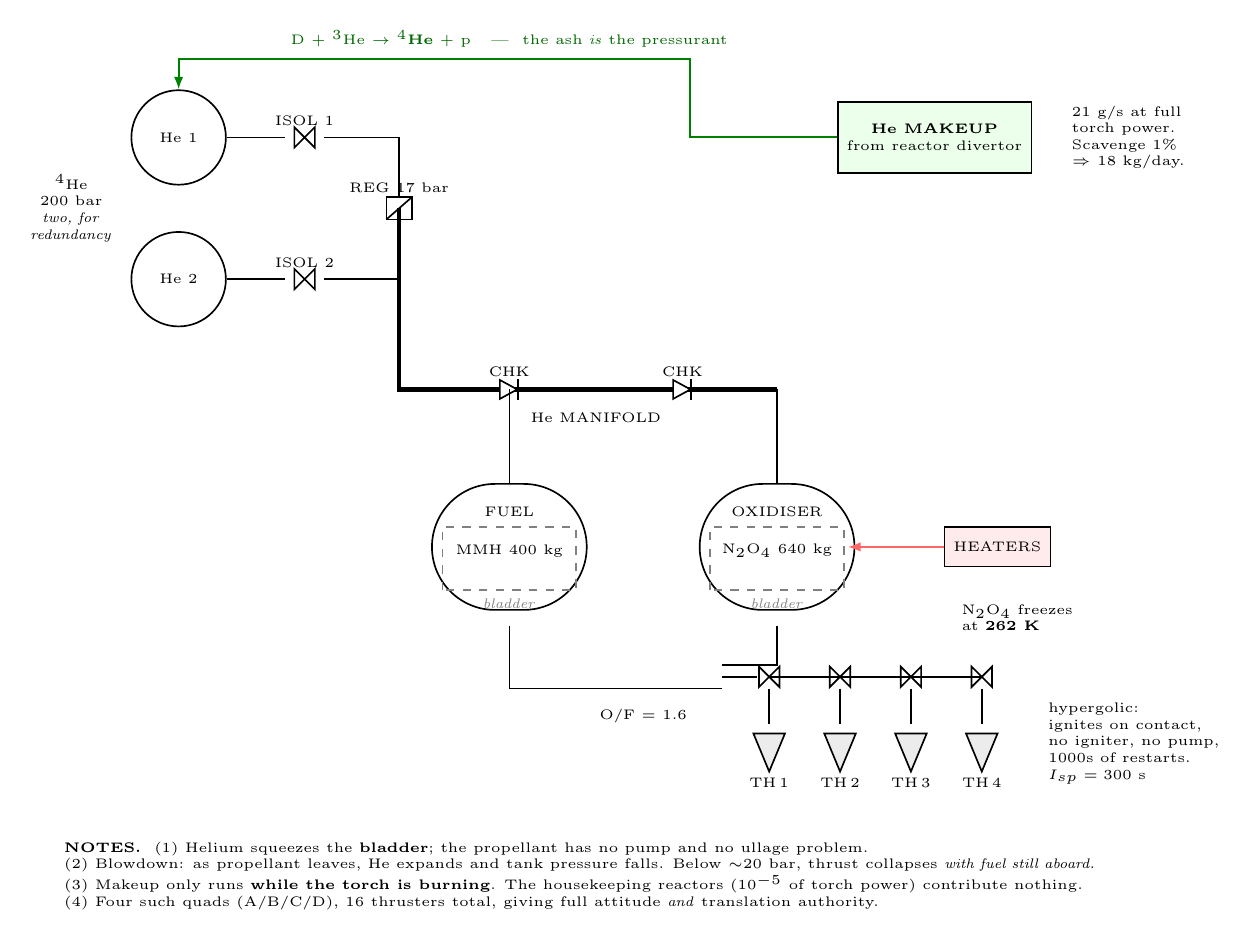
\begin{tikzpicture}[x=1cm,y=1cm]
% helium bottles
\node[sph,minimum size=12mm] (H1) at (0,4.6) {He 1};
\node[sph,minimum size=12mm] (H2) at (0,2.8) {He 2};
\node[lbl,align=center,anchor=east] at (-0.8,3.7) {$^4$He\\200 bar\\\emph{two, for}\\\emph{redundancy}};
% isolation valves
\valve{1.6}{4.6}{ISOL 1}   \valve{1.6}{2.8}{ISOL 2}
\draw (H1.east) -- (1.35,4.6);  \draw (1.85,4.6) -- (2.8,4.6) -- (2.8,3.9);
\draw (H2.east) -- (1.35,2.8);  \draw (1.85,2.8) -- (2.8,2.8) -- (2.8,3.5);
% regulator
\reg{2.8}{3.7}{REG 17 bar}
\draw (2.8,3.5) -- (2.8,3.56);
\draw (2.8,3.84) -- (2.8,4.4);
% manifold to both prop tanks
\draw[bus] (2.8,3.7) -- (2.8,1.4) -- (7.6,1.4);
\chk{4.2}{1.4}{CHK}  \chk{6.4}{1.4}{CHK}
\node[lbl,below] at (5.3,1.15) {He MANIFOLD};
% propellant tanks with bladders
\node[tank,minimum width=22mm,minimum height=16mm] (FU) at (4.2,-0.6) {};
\node[lbl] at (4.2,-0.15) {FUEL};
\node[lbl] at (4.2,-0.65) {MMH 400 kg};
\draw[dashed,gray] (3.35,-1.15) rectangle (5.05,-0.35);
\node[lbl,gray] at (4.2,-1.32) {\emph{bladder}};
\node[tank,minimum width=22mm,minimum height=16mm] (OX) at (7.6,-0.6) {};
\node[lbl] at (7.6,-0.15) {OXIDISER};
\node[lbl] at (7.6,-0.65) {N$_2$O$_4$ 640 kg};
\draw[dashed,gray] (6.75,-1.15) rectangle (8.45,-0.35);
\node[lbl,gray] at (7.6,-1.32) {\emph{bladder}};
\draw (4.2,1.4) -- (4.2,0.2);
\draw (7.6,1.4) -- (7.6,0.2);
% heaters
\node[blk,minimum width=10mm,minimum height=5mm,fill=red!8] (HT) at (10.4,-0.6) {HEATERS};
\draw[flow,red!60] (HT.west) -- (8.5,-0.6);
\node[lbl,align=left,anchor=west] at (9.9,-1.5) {N$_2$O$_4$ freezes\\at \textbf{262 K}};
% feed to thrusters
\draw (4.2,-1.6) -- (4.2,-2.4) -- (6.9,-2.4);
\draw (7.6,-1.6) -- (7.6,-2.1) -- (6.9,-2.1);
\node[lbl,align=center] at (5.9,-2.75) {O/F = 1.6};
% thruster valves + 4 thrusters
\foreach \i in {0,1,2,3}{
  \valve{7.5+0.9*\i}{-2.25}{}
  \node[thr,fill=gray!15,shape border rotate=270] at (7.5+0.9*\i,-3.1) {};
  \node[lbl] at (7.5+0.9*\i,-3.6) {TH\,\number\numexpr\i+1\relax};
  \draw (7.5+0.9*\i,-2.4) -- (7.5+0.9*\i,-2.85);
}
\draw (6.9,-2.25) -- (7.35,-2.25);
\draw (7.5,-2.25) -- (10.2,-2.25);
\node[lbl,align=left,anchor=west] at (11.0,-3.1) {hypergolic:\\ignites on contact,\\no igniter, no pump,\\1000s of restarts.\\$I_{sp}=300$ s};
% helium makeup from reactor
\node[blk,minimum width=24mm,minimum height=9mm,fill=green!8] (MK) at (9.6,4.6)
  {\textbf{He MAKEUP}\\from reactor divertor};
\draw[flow,green!50!black] (MK.west) -- (6.5,4.6) -- (6.5,5.6) -- (0,5.6) -- (H1.north);
\node[lbl,green!40!black,align=center] at (4.2,5.85) {D + $^3$He $\to$ \textbf{$^4$He} + p \ \ ---\ \ the ash \emph{is} the pressurant};
\node[lbl,align=left,anchor=west] at (11.3,4.6) {21 g/s at full\\torch power.\\Scavenge 1\%\\$\Rightarrow$ 18 kg/day.};
% notes
\node[lbl,align=left,anchor=north west] at (-1.5,-4.3)
 {\textbf{NOTES.}\ \ (1) Helium squeezes the \textbf{bladder}; the propellant has no pump and no ullage problem.\\
  (2) Blowdown: as propellant leaves, He expands and tank pressure falls. Below $\sim$20 bar, thrust collapses \emph{with fuel still aboard}.\\
  (3) Makeup only runs \textbf{while the torch is burning}. The housekeeping reactors ($10^{-5}$ of torch power) contribute nothing.\\
  (4) Four such quads (A/B/C/D), 16 thrusters total, giving full attitude \emph{and} translation authority.};
\end{tikzpicture}
\end{center}

\section{Electrical power (EPS)}

\begin{center}
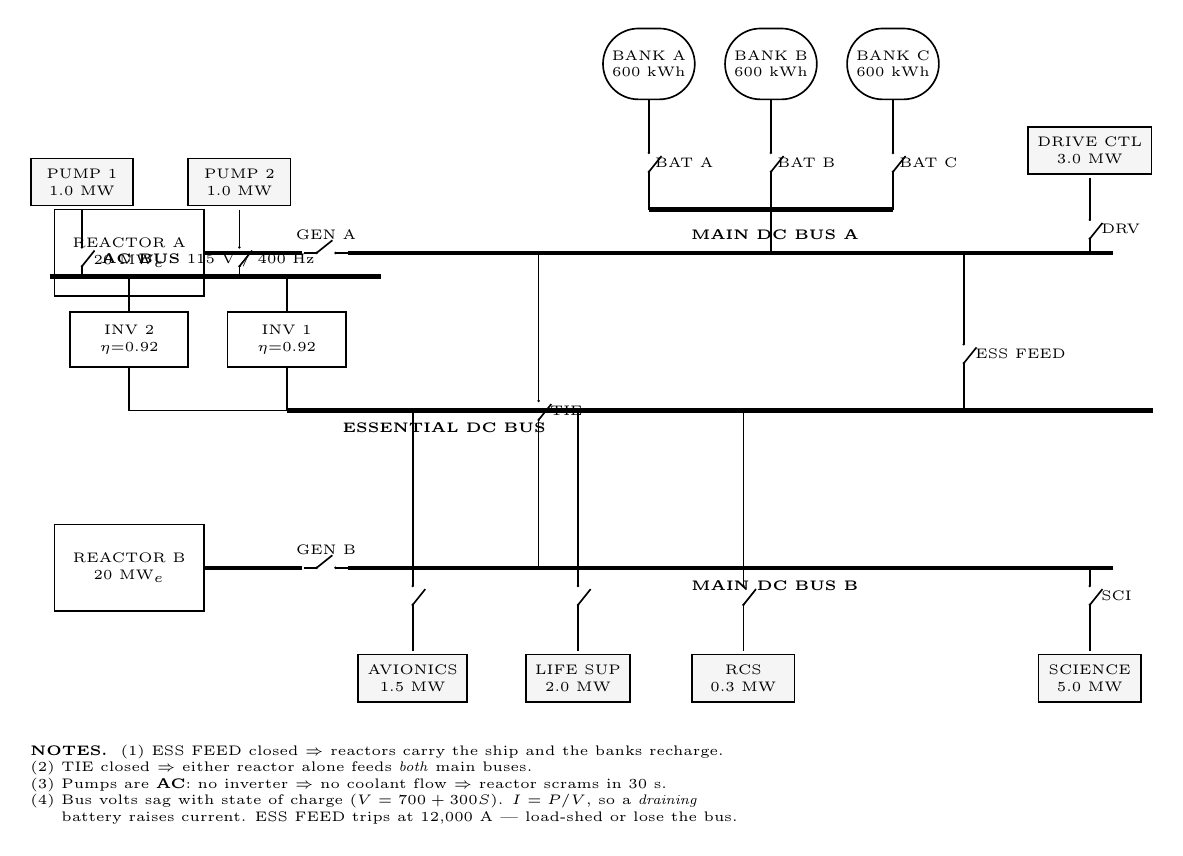
\begin{tikzpicture}[x=1cm,y=1cm]
% --- reactors ---
\node[blk,minimum height=11mm,minimum width=19mm] (RA) at (0,4) {REACTOR A\\20 MW$_e$};
\node[blk,minimum height=11mm,minimum width=19mm] (RB) at (0,0) {REACTOR B\\20 MW$_e$};
% --- gen breakers ---
\draw[bus] (RA.east) -- (2.2,4);   \cbH{2.5}{4}{GEN A}
\draw[bus] (RB.east) -- (2.2,0);   \cbH{2.5}{0}{GEN B}
\draw[bus] (2.78,4) -- (4,4);
\draw[bus] (2.78,0) -- (4,0);
% --- main buses ---
\draw[bus] (4,4) -- (12.5,4);  \node[lbl,above] at (8.2,4.12) {\textbf{MAIN DC BUS A}};
\draw[bus] (4,0) -- (12.5,0);  \node[lbl,below] at (8.2,-0.12) {\textbf{MAIN DC BUS B}};
% --- tie ---
\draw (5.2,4) -- (5.2,2.28);  \cbV{5.2}{2}{TIE}
\draw (5.2,1.72) -- (5.2,0);
% --- battery banks ---
\foreach \i/\n in {0/A,1/B,2/C}{
  \node[tank,minimum width=14mm] (BK\n) at (6.6+1.55*\i,6.4) {BANK \n\\600 kWh};
  \draw (6.6+1.55*\i,5.95) -- (6.6+1.55*\i,5.4);
  \cbV{6.6+1.55*\i}{5.15}{}
  \node[lbl] at (7.05+1.55*\i,5.15) {BAT \n};
  \draw (6.6+1.55*\i,4.9) -- (6.6+1.55*\i,4.55);
}
\draw[bus] (6.6,4.55) -- (9.7,4.55);
\draw (8.15,4.55) -- (8.15,4);
% --- ESS feed ---
\draw (10.6,4) -- (10.6,3.0); \cbV{10.6}{2.72}{ESS FEED}
\draw (10.6,2.44) -- (10.6,2.0);
\draw[bus] (2.0,2.0) -- (13.0,2.0);
\node[lbl,below] at (4.0,1.88) {\textbf{ESSENTIAL DC BUS}};
% --- inverters -> AC bus ---
\node[blk] (I1) at (2.0,2.9) {INV 1\\$\eta$=0.92};
\node[blk] (I2) at (0.0,2.9) {INV 2\\$\eta$=0.92};
\draw (2.0,2.0) -- (2.0,2.55);
\draw (0.0,2.55) -- (0.0,2.0) -- (2.0,2.0);
\draw[bus] (-1.0,3.7) -- (3.2,3.7);
\node[lbl,above] at (1.0,3.78) {\textbf{AC BUS} 115 V / 400 Hz};
\draw (2.0,3.25) -- (2.0,3.7);
\draw (0.0,3.25) -- (0.0,3.7);
% --- AC loads: pumps ---
\node[load] (P1) at (-0.6,4.9) {PUMP 1\\1.0 MW};
\node[load] (P2) at (1.4,4.9) {PUMP 2\\1.0 MW};
\draw (-0.6,4.55) -- (-0.6,4.15); \cbV{-0.6}{3.95}{}
\draw (1.4,4.55) -- (1.4,4.15);   \cbV{1.4}{3.95}{}
% --- DC loads on ESS ---
\foreach \i/\n/\p in {0/AVIONICS/1.5, 1/LIFE SUP/2.0, 2/RCS/0.3}{
  \node[load] (L\i) at (3.6+2.1*\i,-1.4) {\n\\\p\ MW};
  \draw (3.6+2.1*\i,-1.05) -- (3.6+2.1*\i,-0.55);
  \cbV{3.6+2.1*\i}{-0.35}{}
  \draw (3.6+2.1*\i,-0.1) -- (3.6+2.1*\i,2.0);
}
% --- MAIN-BUS-ONLY loads ---
\node[load] (DRV) at (12.2,5.3) {DRIVE CTL\\3.0 MW};
\node[load] (SCI) at (12.2,-1.4) {SCIENCE\\5.0 MW};
\draw (12.2,4.95) -- (12.2,4.55); \cbV{12.2}{4.3}{DRV}
\draw (12.2,4.05) -- (12.2,4);
\draw (12.2,-1.05) -- (12.2,-0.55); \cbV{12.2}{-0.35}{SCI}
\draw (12.2,-0.1) -- (12.2,0);
% notes
\node[lbl,align=left,anchor=north west] at (-1.3,-2.2)
 {\textbf{NOTES.}\ \ (1) ESS FEED closed $\Rightarrow$ reactors carry the ship and the banks recharge.\\
  (2) TIE closed $\Rightarrow$ either reactor alone feeds \emph{both} main buses.\\
  (3) Pumps are \textbf{AC}: no inverter $\Rightarrow$ no coolant flow $\Rightarrow$ reactor scrams in 30 s.\\
  (4) Bus volts sag with state of charge ($V=700+300S$). $I=P/V$, so a \emph{draining}\\
  \phantom{(4) }battery raises current. ESS FEED trips at 12{,}000 A --- load-shed or lose the bus.};
\end{tikzpicture}
\end{center}

The bus is a network of stores and converters. With battery state $E$:
\begin{equation}
\frac{dE}{dt}=P_{\text{gen}}-P_{\text{load}},\qquad 0\le E\le E_{\max},
\qquad I=\frac{P}{V}.
\end{equation}
Two design details drive all the gameplay:

\textbf{Voltage sag.} Battery terminal voltage falls with state of charge, modelled linearly as $V=700+300\,S$ volts. Since $I=P/V$, \emph{a draining battery draws more current for the same load}. Push the essential bus past its 12{,}000 A breaker rating during a cold start and it trips --- a genuine emergent failure, not a scripted one.

\textbf{Inverter losses are heat.} Pumps are AC; the inverter is $\eta=0.92$, so DC draw is $P_{\text{AC}}/\eta$ and the missing $8\%$ lands in the coolant loop. Conservation of energy means \textbf{every watt consumed anywhere becomes heat you must radiate.}

\section{Thermal control}

\begin{center}
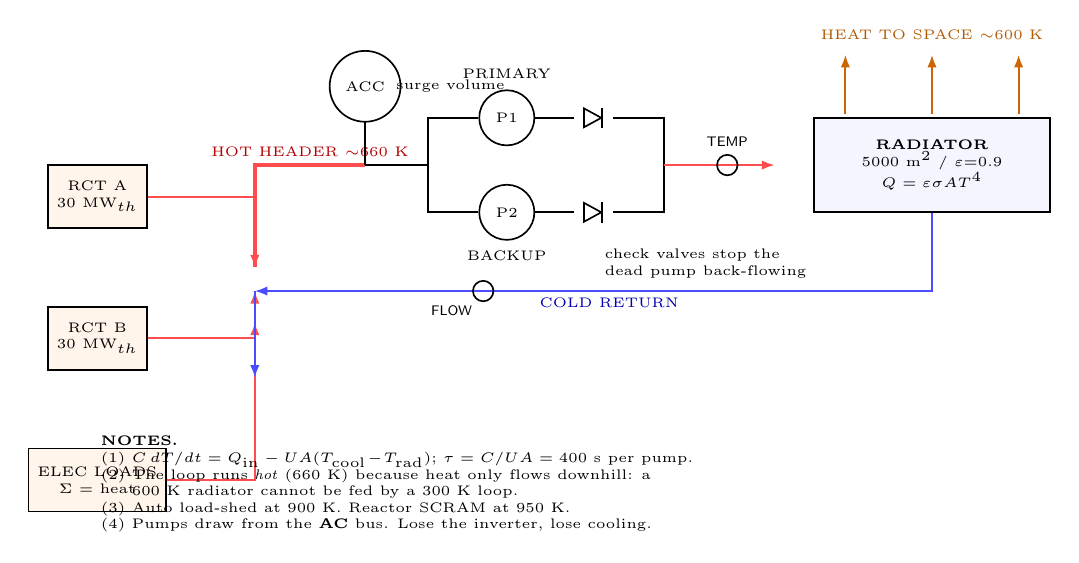
\begin{tikzpicture}[x=1cm,y=1cm]
% reactors as heat sources
\node[hx] (RA) at (0,3.2) {RCT A\\30 MW$_{th}$};
\node[hx] (RB) at (0,1.4) {RCT B\\30 MW$_{th}$};
\node[hx,minimum width=14mm] (EL) at (0,-0.4) {ELEC LOADS\\$\Sigma$ = heat};
% hot header
\draw[flow,red!70] (RA.east) -- (2.0,3.2) -- (2.0,2.3);
\draw[flow,red!70] (RB.east) -- (2.0,1.4) -- (2.0,2.0);
\draw[flow,red!70] (EL.east) -- (2.0,-0.4) -- (2.0,1.6);
\draw[bus,red!70] (2.0,2.3) -- (2.0,3.6) -- (3.4,3.6);
\node[lbl,red!70!black,above] at (2.7,3.66) {HOT HEADER $\sim$660 K};
% accumulator
\node[sph] (ACC) at (3.4,4.6) {ACC};
\draw (3.4,4.15) -- (3.4,3.6);
\node[lbl,right] at (3.75,4.6) {surge volume};
% pumps in parallel
\node[pump] (P1) at (5.2,4.2) {P1};
\node[pump] (P2) at (5.2,3.0) {P2};
\draw (3.4,3.6) -- (4.2,3.6) -- (4.2,4.2) -- (P1.west);
\draw (4.2,3.6) -- (4.2,3.0) -- (P2.west);
\node[lbl,above=1mm] at (5.2,4.55) {PRIMARY};
\node[lbl,below=1mm] at (5.2,2.65) {BACKUP};
% check valves after pumps
\chk{6.3}{4.2}{} \chk{6.3}{3.0}{}
\draw (P1.east) -- (6.05,4.2);  \draw (6.55,4.2) -- (7.2,4.2) -- (7.2,3.6);
\draw (P2.east) -- (6.05,3.0);  \draw (6.55,3.0) -- (7.2,3.0) -- (7.2,3.6);
\node[lbl,align=left,anchor=west] at (6.4,2.35) {check valves stop the\\dead pump back-flowing};
% to radiator
\draw[flow,red!70] (7.2,3.6) -- (8.6,3.6);
\node[rad,minimum width=30mm,minimum height=12mm] (RAD) at (10.6,3.6)
  {\textbf{RADIATOR}\\5000 m$^2$ / $\varepsilon$=0.9\\$Q=\varepsilon\sigma A T^4$};
% radiated heat
\foreach \x in {9.5,10.6,11.7}{\draw[flow,orange!80!black] (\x,4.25) -- (\x,5.0);}
\node[lbl,orange!70!black] at (10.6,5.25) {HEAT TO SPACE $\sim$600 K};
% return
\draw[flow,blue!70] (RAD.south) -- (10.6,2.0) -- (2.0,2.0);
\node[lbl,blue!70!black,below] at (6.5,1.95) {COLD RETURN};
\draw[flow,blue!70] (2.0,2.0) -- (2.0,0.9);
% sensors
\node[lbl] at (8.0,3.9) {\textsf{TEMP}};
\draw (8.0,3.6) circle (0.13);
\node[lbl] at (4.5,1.75) {\textsf{FLOW}};
\draw (4.9,2.0) circle (0.13);
% notes
\node[lbl,align=left,anchor=north west] at (0,0.2)
 {\textbf{NOTES.}\\
  (1) $C\,dT/dt = Q_{\text{in}} - UA(T_{\text{cool}}\!-\!T_{\text{rad}})$; $\tau = C/UA = 400$ s per pump.\\
  (2) The loop runs \emph{hot} (660 K) because heat only flows downhill: a\\
  \phantom{(2) }600 K radiator cannot be fed by a 300 K loop.\\
  (3) Auto load-shed at 900 K. Reactor SCRAM at 950 K.\\
  (4) Pumps draw from the \textbf{AC} bus. Lose the inverter, lose cooling.};
\end{tikzpicture}
\end{center}

\textbf{Rejection} is Stefan--Boltzmann:
\begin{equation}
\boxed{\;Q_{\text{rad}}=\varepsilon\sigma A\,T^{4}\;}\qquad
T_{\text{eq}}=\left(\frac{Q}{\varepsilon\sigma A}\right)^{1/4}.
\end{equation}
The fourth power is unforgiving: doubling heat load raises radiator temperature only $19\%$, but halving the area demands $19\%$ more temperature. \textbf{Radiators must run hot} --- ORION's housekeeping loop sits near 650--670 K precisely so its radiator (at $\sim$600 K) can shed anything at all. Heat only flows downhill; a 300 K coolant loop cannot push heat into a 700 K radiator.

\textbf{Transport} between loops is a lumped conductance:
\begin{equation}
Q_{\text{pump}}=UA\,(T_{\text{cool}}-T_{\text{rad}}),\qquad
C\frac{dT}{dt}=Q_{\text{in}}-Q_{\text{out}},\qquad \tau=\frac{C}{UA}.
\end{equation}
With $C=2\times10^{8}\unit{J/K}$ and $UA=5\times10^{5}\unit{W/K}$ per pump, $\tau=400\unit{s}$ --- slow enough to fight, fast enough to kill you. \textbf{With no pump running there is no path from the loop to the radiator at all}, and the temperature diverges regardless of load shedding. That is why the pump is redundant.

\begin{center}
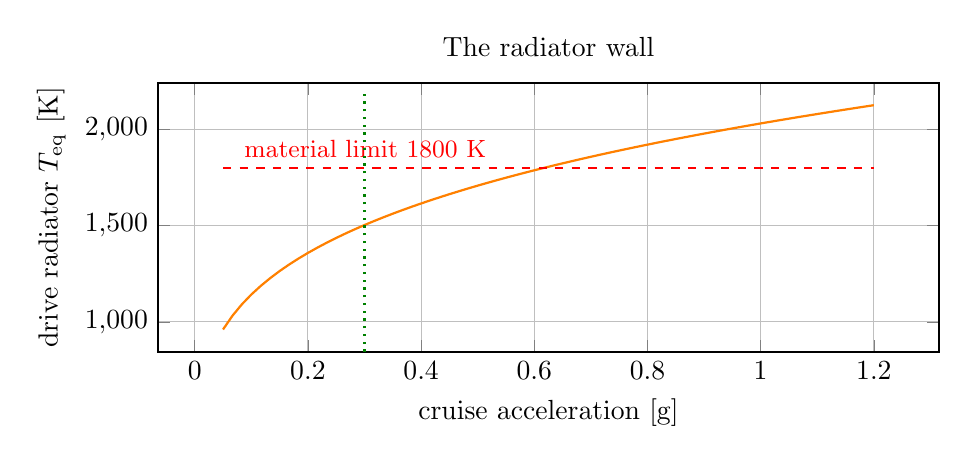
\begin{tikzpicture}
\begin{axis}[width=11.5cm,height=5cm,xlabel={cruise acceleration [g]},ylabel={drive radiator $T_{\text{eq}}$ [K]},
  domain=0.05:1.2,samples=70,grid=both,title={The radiator wall}]
\addplot[thick,orange]{(1.703e13*x)^(0.25)};
\draw[red,dashed,thick](axis cs:0.05,1800)--(axis cs:1.2,1800);
\node[red,anchor=west,font=\small] at (axis cs:0.07,1900){material limit 1800 K};
\draw[green!50!black,dotted,thick](axis cs:0.30,0)--(axis cs:0.30,2200);
\node[green!50!black,rotate=90,anchor=south,font=\tiny] at (axis cs:0.30,300){design 0.30 g};
\end{axis}
\end{tikzpicture}
\end{center}

\section{Mass closure}
Every subsystem's mass feeds $F=ma$, so the ship is a \emph{fixed point}, not a sum:
\begin{align}
m_{\text{drive}}&=\frac{\tfrac12 m_{\text{wet}}\,a\,\ve}{(P/m)_{\text{spec}}}, &
m_{\text{rad}}&=\frac{Q_{\text{waste}}}{\varepsilon\sigma T_{\lim}^{4}}\rho_A,\\
m_{\text{dry}}&=\big(\text{fixed}+m_{\text{drive}}+m_{\text{rad}}+m_{\text{shield}}\big)(1+f_{\text{hull}}), &
m_{\text{prop}}&=m_{\text{dry}}\!\left(e^{\Delta v/\ve}-1\right).
\end{align}
Because $m_{\text{drive}}\propto m_{\text{wet}}$, the loop can diverge. Solving iteratively at $0.30\,\gz$ with a 50 MW/kg drive gives a \textbf{646 t ship}:

\begin{center}
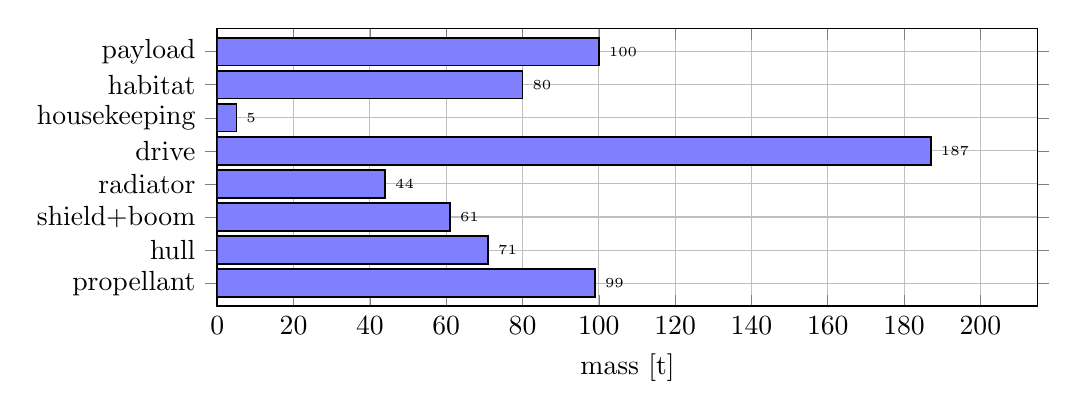
\begin{tikzpicture}
\begin{axis}[width=12cm,height=5cm,xbar,y=0.42cm,
  xlabel={mass [t]},symbolic y coords={propellant,hull,shield+boom,radiator,drive,housekeeping,habitat,payload},
  ytick=data,nodes near coords,nodes near coords style={font=\tiny},xmin=0,xmax=215,grid=major]
\addplot[fill=blue!50] coordinates {(100,payload)(80,habitat)(5,housekeeping)(187,drive)(44,radiator)(61,shield+boom)(71,hull)(99,propellant)};
\end{axis}
\end{tikzpicture}
\end{center}

\noindent The drive is 29\% of the ship. \textbf{Drive specific power is the master constraint}: at 25 MW/kg no ship closes above $0.34\,\gz$; at 50 MW/kg the wall is $0.58\,\gz$; at 100 MW/kg, $0.92\,\gz$. Heat and radiation never get a chance to bind first.

\section{How many nozzles?}
A real design question with a decisive answer. Four arguments \emph{for} splitting the drive, one hard constraint on \emph{how}.

\subsection{For: engine-out survivability --- the strongest argument}
A brachistochrone is uniquely unforgiving. Deceleration must \emph{equal} acceleration: you spend half the trip building 814 km/s and the other half killing it. Lose thrust at the flip and the required decel is exactly $a$ --- \textbf{with less thrust you cannot stop, and you fly past Mars at a substantial fraction of a percent of light speed.}

But if you lose a nozzle \emph{early}, you can flip early and still make it:
\begin{center}\small
\begin{tabular}{@{}lrrr@{}}
\toprule
Nozzles & Thrust & Flip at & Trip time\\
\midrule
4 / 4 & 100\% & 50.0\% of range & 6.40 d\\
3 / 4 & 75\%  & 42.9\% of range & 6.91 d \;(+8\%)\\
2 / 4 & 50\%  & 33.3\% of range & 7.84 d \;(+22\%)\\
1 / 4 & 25\%  & 20.0\% of range & 9.80 d \;(+53\%)\\
\bottomrule
\end{tabular}
\end{center}
\textbf{A single-nozzle ship has no engine-out case at all.} A four-nozzle ship loses one and arrives 8\% late. That alone justifies the split.

\subsection{For: thrust vector control without gimballing}
Gimballing a multi-gigawatt superconducting magnetic nozzle is mechanically absurd. Differential throttling gives steering for free: with four nozzles on a radius $r$, throttling one by 10\% produces
\begin{equation}
\tau = \Delta F \cdot r = (0.10 \times 478\unit{kN})(5\unit{m}) = 239\unit{kN\,m},
\end{equation}
which is \textbf{four times} the torque of an entire RCS quad ($60\unit{kN\,m}$) --- and it costs no RCS propellant, because you are burning anyway.

\subsection{For: throttle turn-down}
A magnetic nozzle has a \emph{minimum} stable plasma flow; below it the plasma will not detach from the field lines. If each nozzle throttles only 40--100\%, then:
\begin{center}\small
\begin{tabular}{@{}lr@{}}
\toprule
Nozzles lit & Total thrust available\\
\midrule
1 & 10--25\%\\ 2 & 20--50\%\\ 3 & 30--75\%\\ 4 & 40--100\%\\
\bottomrule
\end{tabular}
\end{center}
Continuous 10--100\% coverage. A single nozzle could manage only 40--100\%.

\subsection{Against --- and the geometry that dictates the layout}
Costs are real: more coils, more cryogenics, more plasma feeds, more quench-protection circuits, and a worse surface-to-volume ratio (smaller nozzles detach plasma less efficiently).

But the \textbf{decisive} constraint is the shadow shield. The shield works because the drive is a \emph{point} source directly behind the crew. Spread the source over a radius $R_{\text{src}}$ and the penumbra widens the shield:
\begin{equation}
R_{\text{shield}} \;=\; R_{\text{crew}}\frac{x}{L} \;+\; R_{\text{src}}\Bigl(1-\frac{x}{L}\Bigr),
\end{equation}
with $x$ the shield's distance from the source and $L=121$ m the boom. Shield \emph{mass} scales as $R_{\text{shield}}^2$:

\begin{center}
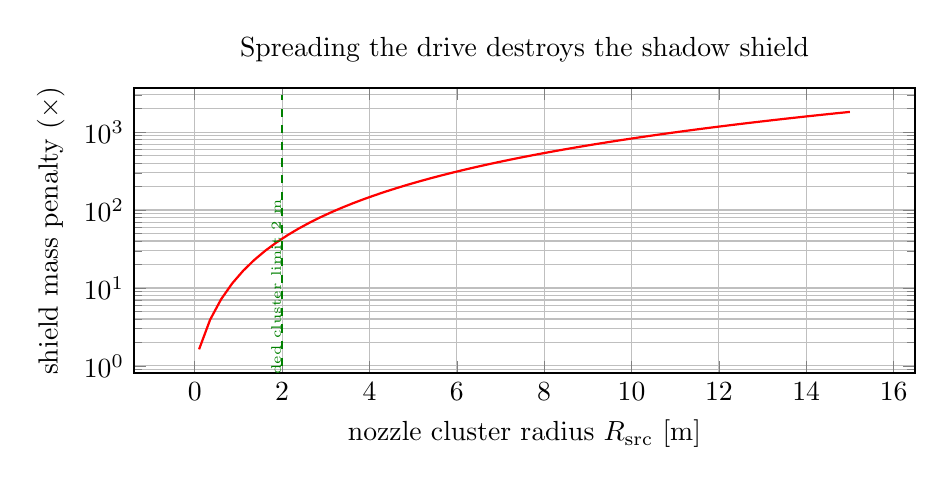
\begin{tikzpicture}
\begin{axis}[width=11.5cm,height=5.2cm,ymode=log,
  xlabel={nozzle cluster radius $R_{\text{src}}$ [m]},
  ylabel={shield mass penalty ($\times$)},
  grid=both,domain=0.1:15,samples=60,title={Spreading the drive destroys the shadow shield}]
\addplot[thick,red]{((4*(10/121) + x*(1-10/121))/(4*(10/121)))^2};
\draw[green!50!black,dashed,thick](axis cs:2,1)--(axis cs:2,3000);
\node[green!50!black,rotate=90,anchor=south,font=\tiny] at (axis cs:2.2,3){recommended cluster limit 2 m};
\end{axis}
\end{tikzpicture}
\end{center}

\begin{center}\small
\begin{tabular}{@{}rrr@{}}
\toprule
$R_{\text{src}}$ & Cluster span & Shield mass penalty\\
\midrule
0 m (point) & --- & $1\times$\\
1 m & 2 m across & $14\times$\\
\textbf{2 m} & \textbf{4 m across} & $\mathbf{43\times}$\\
5 m & 10 m across & $221\times$\\
15 m & 30 m across & $1817\times$\\
\bottomrule
\end{tabular}
\end{center}

\subsection{Verdict}
\begin{center}\fbox{\parbox{0.93\textwidth}{\centering
\textbf{Four nozzles, tightly clustered on the centreline ($R_{\text{src}} \le 2$ m).}\\[3pt]
You buy engine-out survival, gimbal-free thrust vectoring, and a 10--100\% throttle range.\\
You pay in coil mass and complexity --- but \emph{only if you keep them close}.\\
Spread them across the aft end for a prettier silhouette and the shadow shield eats the ship.}}
\end{center}

\noindent The shield penalty is the reason real nuclear-electric designs cluster their engines, and it is a satisfying constraint: the \emph{radiation} problem, not the propulsion problem, dictates the engine layout.


\section{Navigation summary}
Detailed derivations are in the companion document; the operational summary:
\begin{center}\small
\begin{tabular}{@{}lrrrr@{}}
\toprule
Route & Mode & $\Delta v$ & Time & Note\\
\midrule
Earth$\to$Moon & torch $0.30\gz$ & 67 km/s & \textbf{6.3 h} & straight line\\
Earth$\to$Moon & ballistic (TLI) & 3.14 km/s & 5.0 d & Apollo-like\\
Earth$\to$Mars & torch $0.30\gz$ & 1627 km/s & \textbf{6.4 d} & brachistochrone\\
Earth$\to$Mars & Hohmann & 5.59 km/s & 259 d & 780 d synodic wait\\
\bottomrule
\end{tabular}
\end{center}
Guidance uses a universal-variable \textbf{Lambert} solver (Stumpff functions, bisection on $z$) for arbitrary flight times, and an iterative intercept solver for the brachistochrone, since the target moves during transit. Note that $\Delta\nu=180^\circ$ is a genuine \emph{singularity} of Lambert's problem --- the transfer plane is undefined --- and the solver correctly refuses it.

\section{Systems to build next}
\begin{enumerate}\itemsep2pt
\item \textbf{Direct energy conversion} --- charged-product power recovery at $\eta\approx0.7$, as an alternative to the thermal cycle; changes the waste-heat budget dramatically.
\item \textbf{Magnetic nozzle} --- throat field strength, detachment efficiency, and a failure mode where the plasma fails to detach and scours the nozzle.
\item \textbf{Fuel cryogenics} --- D/\he\ storage, boil-off, and the tritium bred from D--D side reactions.
\item \textbf{Neutron activation} --- structure becomes radioactive over mission life; a maintenance-and-dose mechanic.
\item \textbf{Life support \& consumables} --- O$_2$/CO$_2$/H$_2$O, already prototyped in the LCARS build.
\item \textbf{Optics subsystem} --- sextant and scanning telescope, so star marks are \emph{flown} rather than assumed.
\item \textbf{Comms} --- Friis link budget, light-lag; prototyped, not yet ported.
\end{enumerate}

\section{Programme plan}
\textbf{Decision taken:} build as an \textbf{Orbiter 2024 addon} (MIT-licensed, n-body Newtonian, VSOP87/ELP2000 ephemerides). Orbiter supplies orbital mechanics and rendering; we supply the ship.

\textbf{Architectural rule:} \texttt{ShipCore} has \emph{zero} Orbiter dependencies. It compiles and unit-tests standalone; \texttt{Orion.cpp} (a \texttt{VESSEL4} subclass) is thin glue with no physics in it. We never reimplement orbital mechanics.

\begin{center}\small
\begin{tabular}{@{}llp{7.4cm}@{}}
\toprule
Phase & Status & Content\\
\midrule
0. Physics core & \textbf{done} & Propulsion, thermal, shielding, mass closure --- validated in Python\\
1. Interactive prototypes & \textbf{done} & Browser consoles: cold-start, systems, LCARS, GN\&C\\
2. Navigation & \textbf{done} & Lambert (0.00 km miss verified), brachistochrone, Hohmann windows\\
3. \texttt{ShipCore} in C++ & \textbf{done} & Reactor/EPS/ECS, 6/6 unit tests passing, engine-agnostic\\
4. Orbiter vessel & \emph{in progress} & \texttt{VESSEL4} glue, fixed-timestep substepping, scenario persistence\\
5. Nav MFD & \emph{in progress} & Lambert + brachistochrone targeting on Orbiter's state vector\\
6. 2D panel & see below & Clickable breakers, reactor gauges --- the \emph{Reentry} feel\\
7. Mass augmentation & \textbf{done} & Mixing valve in \texttt{ShipCore}; 9/9 tests passing\\
8. Avionics & \textbf{done} & IMU + gimbal lock, P52 (4 options, scheduled), GDC, RCS quads\\
9. 2D panel & \textbf{next} & Clickable breakers, reactor gauges, FDAI\\
10. Virtual cockpit & planned & 3D panel, mesh, switches\\
\bottomrule
\end{tabular}
\end{center}

\subsection*{Known hazards for phase 4--5}
\begin{itemize}\itemsep0pt
\item Orbiter's \texttt{simdt} reaches hundreds of seconds under time acceleration. \textbf{Never} feed it to an ODE integrator --- accumulate and substep at fixed 0.1 s.
\item The addon DLL is \emph{not} unloaded between scenarios; global mutable state leaks into the next flight.
\item Orbiter's \texttt{Isp} argument to \texttt{CreateThruster} is exhaust velocity in \textbf{m/s}, not seconds. Pass $9.81\times10^{6}$ directly.
\item Thruster handles must be created in \texttt{clbkSetClassCaps}; touching them earlier is a crash-to-desktop.
\item The mixing valve changes $\ve$ \emph{at runtime}, so \texttt{Orion.cpp} must call \texttt{SetThrusterIsp()} every step --- a thruster's $I_{sp}$ is not fixed once created.
\end{itemize}

\end{document}
